\section{Experiments}
\label{sec:exploring-boundaries:Experiments}
We performed a number of experiments to determine the size of the state space of intermediate models generated by sequences of refining transformations.
By transforming intermediate \SLCO models to \Promela models, we obtain models whose state space can be explored using \Spin.
For the experiments described below, we configured Spin to explore the state-spaces by means of a depth-first search with a maximum search depth of $ 1\cdot10^8$ transitions and using at most $4\cdot10^4$ megabytes of memory.
After describing the models that serve as inputs in our experiment, we show that an approach using coarse-grained sequences of transformations quickly leads to models with very large state spaces.
Then, we present the results of our experiments using fine-grained sequences.
Finally, we discuss how applying transformations to a part of the applicable model elements only can also be used to explore the state space of less abstract versions of models.

\subsection{Cases}
We apply the refining transformations described in Section~\ref{sec:exploring-boundaries:comparison-of-transformations} to three different models.
The first model consists of one object that repeatedly sends signals via its port (the producer) and one object that is always able to receive signals via its port (the consumer).
A synchronous channel connects the ports of the producer to the ports of the consumer.
The communication and behavior diagram of this model are shown in Figure~\ref{fig:exploring-boundaries:prod-con}.
In a number of steps, channel~\SLCOChannel{c} is replaced by asynchronous, lossy channels.

\begin{figure}[hbt]
  \centering
  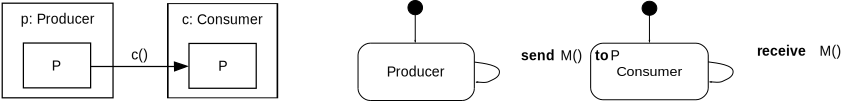
\includegraphics[scale=0.45]{exploring-boundaries/figs/producer-consumer}
  \caption{A producer and a consumer}
  \label{fig:exploring-boundaries:prod-con}
\end{figure}

The second model describes the behavior of a system consisting of three interoperating conveyor belts.
It is a variant of the model described in Section~\ref{sec:slco:sequences} that is obtained by merging the objects~\SLCOObject{Left} and~\SLCOObject{Right}, and subsequently merging the channels that connect them to object~\SLCOObject{Middle}.
The communication diagram of this model is shown in Figure~\ref{fig:exploring-boundaries:conveyor-merge-communication}, and the behavior diagram is shown in Figure~\ref{fig:exploring-boundaries:conveyor-merged-sms}.
The names of the channels are omitted from the communication diagram to increase its readability.
The state machine on the right of Figure~\ref{fig:exploring-boundaries:conveyor-merged-sms} specifies the behavior of object~\SLCOObject{Middle}, and the behavior of object~\SLCOObject{L\_R} is specified using two instances of the state machine shown on the left of the figure.
The third component, which models the environment of the system, is not described here.
This model is transformed by replacing the synchronous channel that connects object~\SLCOObject{L\_R} and object~\SLCOObject{Middle} by asynchronous, lossy channels.

\begin{figure}[hbt]
 \centering
 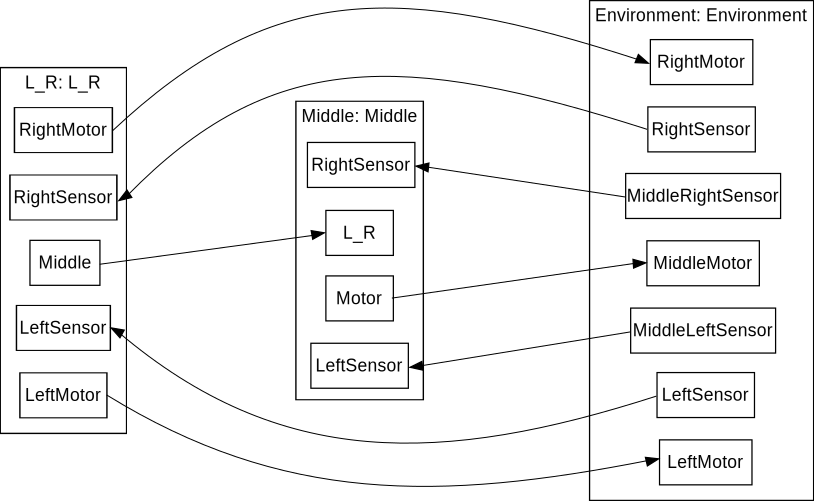
\includegraphics[scale=0.45]{exploring-boundaries/figs/ConveyorExampleCommunicationMerged}
 \caption{Communication diagram of the second model}
 \label{fig:exploring-boundaries:conveyor-merge-communication}
\end{figure}

\begin{figure}[hbt]
 \centering
 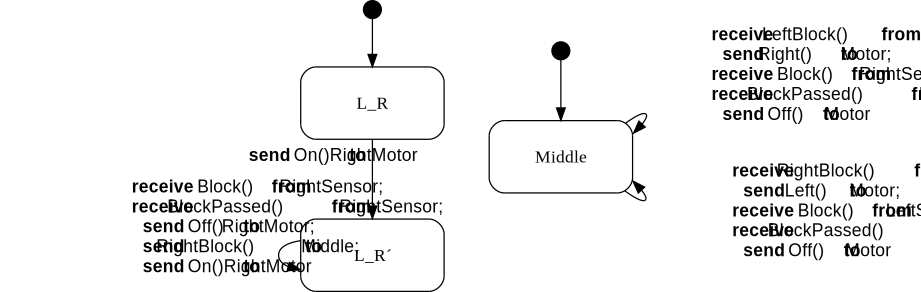
\includegraphics[scale=0.45]{exploring-boundaries/figs/ConveyorExampleSMSMerge}
 \caption{State machines of the second model}
 \label{fig:exploring-boundaries:conveyor-merged-sms}
\end{figure}

The third model consists of two objects that repeatedly send signals via their ports (the producers) and one object that is always able to receive signals via two ports (the consumer).
Two synchronous channels connect the ports of each of the producers to the ports of the consumer.
Figure~\ref{fig:exploring-boundaries:prods-con} shows the communication and behavior diagram of this model.
For the experiments, both channels are replaced by asynchronous, lossy channels.

\begin{figure}[hbt]
  \centering
  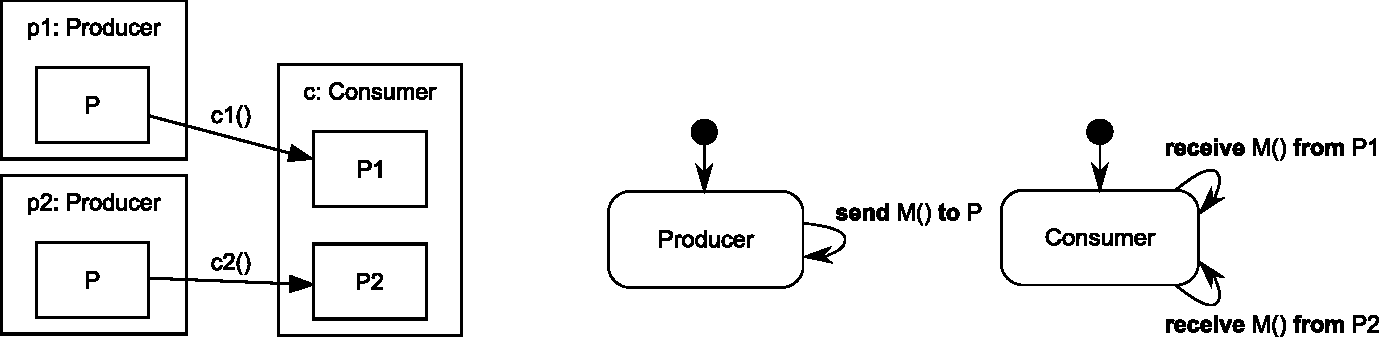
\includegraphics[scale=0.45]{exploring-boundaries/figs/producers-consumer}
  \caption{Two producers and a consumer}
  \label{fig:exploring-boundaries:prods-con}
\end{figure}

For the experiments described in this section, we used a slightly modified version of \SLCO.
In this version of the language, the solid black dots represent the initial states, whereas in the current version of \SLCO described in Chapter~\ref{chap:SLCO}, they do not.
Instead, the dots and their outgoing arrows are currently only used to indicate the initial states.
For the model shown in Figure~\ref{fig:exploring-boundaries:prod-con}, for example, the fact that the black dots represent the initial states themselves means that both the producer and the consumer consist of two states.
This is reflected by the tables in the following section.
The reason for this difference between the older version of \SLCO and the current version is discussed in Chapter~\ref{chap:iterative-dsl-evolution}.

\subsection{Results}
\label{subsec:exploring-boundaries:results}
Applying a coarse-grained sequence of transformations to the model of the producer and consumer leads to the state space sizes shown in Table~\ref{tab:simple_coarse_grained}.
The table shows that replacing synchronous communication by asynchronous communication approximately doubles the size of the state space.
Adding a number of state machines that implement the ABP to each of the two objects, however, leads to a significant increase of the size of the state space.
Although the resulting state space of the most concrete model is much larger than the one of the intermediate model, it is still small enough for verification given the aforementioned configuration of Spin.

\begin{table}[hbt]
\centering
\small
\begin{tabular}{|l|r|r|}
\hline
\rowcolor[gray]{.9}
\textbf{Model}          & \textbf{\# States}      & \textbf{\# Transitions} \\
\hline
 Original               & 4              & 6 \\
\hline
 Asynchronous signals   & 8              & 11 \\
\hline
 Lossless communication & $76\;066\;432$ & $542\;196\;960$ \\
\hline
\end{tabular}
\caption{Coarse-grained sequence applied to the producer and consumer}
\label{tab:simple_coarse_grained}
\end{table}

To further illustrate the effects of coarse-grained sequences of transformations on the size of the state space, we applied one to the second model, which is slightly more complex than the first.
One of the components in the system of the three conveyor belts consists of two instances of the same state machine.
Both instances communicate over the same port, which means that a token server must be added when refining this model, before the transformation that adds the ABP can be employed.
Table~\ref{tab:legocase_coarse_grained} shows that adding a token server leads to a state space that can still be model checked.
The final row in the table indicates that it is impossible to explore the entire state space before the search depth is exceeded or all available memory is used.
This shows that the output of this transformation is not suited for model checking, even though the input model is still relatively small.

\begin{table}[hbt]
\centering
\small
\begin{tabular}{|l|r|r|}
\hline
\rowcolor[gray]{.9}
 \textbf{Model}         & \textbf{\# States} & \textbf{\# Transitions} \\
\hline
 Original               & 494                & $1\;294$ \\
\hline
 Asynchronous signals   & 748                & $1\;980$ \\
\hline
 Token server           & $10\;090$          & $33\;820$ \\
\hline
 Lossless communication & --                 & -- \\
 \hline
\end{tabular}
\caption{Coarse-grained sequence applied to the interoperating conveyor belts}
\label{tab:legocase_coarse_grained}
\end{table}

The results of these experiments led us to implement the versions of the transformations discussed in Section~\ref{subsec:exploring-boundaries:fg_model_transformations}.
Table~\ref{tab:simple_fine_grained} shows the effect of a fine-grained sequence of transformations on the size of the state spaces of the intermediate models in the case of the producer and the consumer, and Table~\ref{tab:legocase_fine_grained} shows the effect in the case of the three interoperating conveyor belts.
The transformations that ensure that all signals have a fixed name, replace bidirectional channels by two unidirectional channels, ensure that each state machine within an object communicates with the ABP over an exclusive channel, and replace strings by integers have no effect on the size of the state space.

%Table~\ref{tab:legocase_fine_grained} shows that the state space of the most concrete model is smaller that the state space of the intermediate model that precedes it.
%This is because one of the strings in this intermediate model is replaced by $0$ and variables have the initial value $0$ by default.
%One of the variables in the most concrete model is initialized to $0$ and each assignment assigns the value $0$ to it.
%In the intermediate model that precedes the most concrete model, however, this variable is assigned a value of type mtype that differs from $0$.
%This leads to a state change that is no longer present in the most concrete model after the last refinement.

\begin{table}[hbt]
\centering
\small
\begin{tabular}{|l|r|r|}
\hline
\rowcolor[gray]{.9}
 \textbf{Model}              & \textbf{\# States} & \textbf{\# Transitions} \\
\hline
 Original                    & 4                  & 6 \\
\hline
 Asynchronous signals        & 8                  & 11 \\
\hline
 Fixed signal names          & 8                  & 11 \\
\hline
 Unidirectional channels     & 8                  & 11 \\
\hline
 Lossless communication      & $114\;388$         & $596\;367$ \\
\hline
 Delays                      & $1\;009\;856$      & $5\;902\;673$ \\
\hline
 Merged objects              & $83\;251\;840$     & $592\;242\;910$ \\
\hline
 Integers instead of strings & $83\;251\;840$     & $592\;242\;910$ \\
\hline
\end{tabular}
\caption{Fine-grained sequence applied to the producer and consumer}
\label{tab:simple_fine_grained}
\end{table}

\begin{table}[hbt]
\centering
\small
\begin{tabular}{|l|r|r|}
\hline
\rowcolor[gray]{.9}
 \textbf{Model}         & \textbf{\# States} & \textbf{\# Transitions} \\
\hline
 Original               & 494                & $1\;294$ \\
\hline
 Asynchronous signals   & 748                & $1\;980$ \\
\hline
 Fixed signal names     & 748                & $1\;980$ \\
\hline
 Unidirectional channels& 748                & $1\;980$ \\
\hline
 Lossless communication & $19\;148\;872$     & $141\;049\;260$ \\
\hline
 Delays                 & $167\;466\;690$    & $1\;334\;614\;400$ \\
\hline
 Exclusive channels     & $167\;466\;690$    & $1\;334\;614\;400$ \\
\hline
 Merged objects         & --                 & -- \\
\hline
\end{tabular}
\caption{Fine-grained sequence applied to the interoperating conveyor belts}
\label{tab:legocase_fine_grained}
\end{table}

In the case of the producer and the consumer, each intermediate model has a state-space that can be explored given the aforementioned configuration of Spin.
In the case of the conveyor belts, however, merging objects leads to a state-space that is too large to explore.
Even though the most concrete model is still unsuited for model checking, the fine-grained sequence of transformations made it possible to explore an intermediate model that is more concrete than the ones produced using the coarse-grained sequence.

\subsection{Exploring the Boundaries}
In both of the cases mentioned above, only two instances of the ABP are added because communication takes place in two directions between one pair of objects.
Table~\ref{tab:simpledouble_fine_grained} shows the results for the model consisting of two producers and one consumer.
To achieve lossless communication over a lossy channel in this case, four instances of the ABP have to be added, because communication takes place in two directions between two pairs of objects.

\begin{table}[hbt]
\centering
\small
\begin{tabular}{|l|r|r|}
\hline
\rowcolor[gray]{.9}
 \textbf{Model}          & \textbf{\# States} & \textbf{\# Transitions} \\
\hline
 Original                & 8                  & 17 \\
\hline
 Asynchronous signals    & 33                 & 68 \\
\hline
 Fixed signal names      & 33                 & 68 \\
\hline
 Unidirectional channels & 33                 & 68 \\
\hline
 Lossless communication  & --                 & -- \\
\hline
\end{tabular}
\caption{Fine-grained sequence applied to two producers and a consumer}
\label{tab:simpledouble_fine_grained}
\end{table}

Adding four instances of the objects that implement the ABP leads to an explosion of the state space.
This makes it very hard to verify properties of this model using state-space exploration.
Table~\ref{tab:simpledouble_fine_grained_partial} shows the effect of adding an instance of the ABP to respectively one, two, and three channels in the model of two producers and one consumer, while leaving the other channels untouched.

\begin{table}[hbt]
\centering
\small
\begin{tabular}{|l|r|r|}
\hline
\rowcolor[gray]{.9}
 \textbf{Model}             & \textbf{\# States} & \textbf{\# Transitions} \\
\hline
 Original                   & 8                  & 17 \\
\hline
 Asynchronous signals       & 33                 & 68 \\
\hline
 Fixed signal names         & 33                 & 68 \\
\hline
 Unidirectional channels    & 33                 & 68 \\
\hline
 one ABP instance           & $5\;188$           & $21\;335$ \\
\hline
 two ABP instances          & $527\;108$         & $3\;224\;435$ \\
\hline
 three ABP instances        & $105\;715\;260$    & $879\;085\;750$ \\
\hline
\end{tabular}
\caption{Incremental introduction of the ABP}
\label{tab:simpledouble_fine_grained_partial}
\end{table}

By replacing communication over only a subset of the four channels in the model by communication via the ABP, a model is obtained with a state space that is significantly smaller than the state space corresponding to the model in which communication over all channels is replaced.
In this way, verification of a model that resembles the implementation more closely than the original, more abstract, model is possible.
The same approach can be used to merge only some of the objects in the model of the interoperating conveyor belts.
In general, applying a refining transformation to a part of the applicable elements in the model only can be used to model check intermediate models that resemble the implementation as close as possible, in cases where it is impossible to model check the completely refined model. 